%--------PACKAGES----------------
\documentclass[11 pt]{extarticle} %,a4paper
\usepackage[T2A,T1]{fontenc}
\usepackage[utf8]{inputenc}
\usepackage{lmodern}
\usepackage{siunitx}
\usepackage{subcaption}
\usepackage{graphicx,etoolbox,fancybox,mdframed}
\usepackage[percent]{overpic}
\usepackage[a4paper,left=2.5cm,right=2.5cm,top=2.5cm,bottom=2.5cm] {geometry}
\usepackage{amsfonts,amsmath,amssymb,esint,eucal,latexsym,skull} % mathsymbols and symbols
\usepackage{mathtools} %successor of amsmath, some additional functionality
%\usepackage{chngcntr}
\usepackage{multirow}
\usepackage{cancel} %\cancel{x} in math mode OR \cancelto{0}{x}
\usepackage{float}% H Places the float at precisely the location in the LaTeX code
\usepackage{makecell,array} %enable to create multicell and adjust spaces in those cells
\usepackage{setspace}\onehalfspacing %1.5 line spacing
\usepackage[bottom,flushmargin,hang,multiple]{footmisc} %footnote ayarları
\setlength\footnotemargin{10pt} %footnote numara-text boslugu
\usepackage{breqn}%break equation
\numberwithin{equation}{section} %section içinde numaralandır
\usepackage{bm,bbm,textcomp,textgreek} %use bbm with NUMBERS!
\usepackage{afterpage}
%\usepackage{fancyhdr,fourier-orns}
%\renewcommand\headrule{\hrulefill\raisebox{-2.1pt}[10pt][10pt]{\quad\decofourleft \decofourright\quad}\hrulefill}
\usepackage{relsize}%typeset larger or smaller than the surrounding text
%\usepackage{indentfirst}
\setlength{\parindent}{0pt}
\usepackage{authblk,url} %author ve e-mail
\urlstyle{tt}
\usepackage{multicol} %multicolums
\setlength{\columnsep}{1cm} %column separation in 
\usepackage{titlesec}
\usepackage{cite}
\usepackage{empheq}

\newcommand\apjs{The Astrophysical Journal, Supplement}
\newcommand*\widefbox[1]{\fbox{\hspace{2em}#1\hspace{2em}}}
%\begin{empheq}[box=\widefbox]{align}
%\bar{\nabla}^{\mu} \bar{h}_{\mu\nu} = 0
%\end{empheq}

%\begin{subequations}
%	\begin{empheq}[box=\widefbox]{align}
%	\bar{\nabla}^{\mu} \bar{h}_{\mu\nu} & = 0 \\
%	\bar{\nabla}^{\mu} \bar{h}_{\mu\nu} & = 0
%	\end{empheq}
%\end{subequations}
\usepackage[toc,title]{appendix}
\usepackage[titles]{tocloft}
\usepackage[svgnames,usenames, dvipsnames,table]{xcolor}
\usepackage{hyperref}
\hypersetup{
	colorlinks = true,
	linkcolor=RoyalBlue, %OliveGreen %PineGreen %Sepia MidnightBlue
	filecolor=BrickRed,      
	urlcolor=Crimson,%SeaGreen,%cyan,%Goldenrod, %Chocolate,
	citecolor=BrickRed,
	pdftitle={Cosmological Inflation}
	bookmarks=true,
	linktocpage=true,
	%pdfpagemode=FullScreen,
}

\usepackage{tikz}
\usepackage{import}
%\usepackage{tkz-fct}
\usepackage{tcolorbox,wrapfig}
%\usepackage{natbib}
\usepackage{pdfpages,rotating}
\usepackage[usestackEOL]{stackengine}
\usepackage{booktabs}
\usepackage{marginnote}
\setlength{\marginparwidth}{1.3cm}
%\usepackage{layout}
%\usepackage{showframe}
\usepackage{pgfplots}
\pgfplotsset{compat=newest}
%\usepackage[miktex]{gnuplottex}
\usetikzlibrary{arrows}   
%\usepackage{showkeys} %shows labels in pdf output
%\usepackage{showlabels} %shows labels in pdf output
\newcommand\numberthis{\addtocounter{equation}{1}\tag{\theequation}}
\usepackage{lipsum}                     % Dummytext
\usepackage{xargs}                      % Use more than one optional parameter in a new commands
%%%%% TO DO COLOR %%%%%%%%
\usepackage[colorinlistoftodos,prependcaption,textsize=small]{todonotes}
\newcommandx{\unsure}[2][1=]{\todo[linecolor=red,backgroundcolor=red!25,bordercolor=red,#1]{#2}}
\newcommandx{\change}[2][1=]{\todo[linecolor=blue,backgroundcolor=blue!25,bordercolor=blue,#1]{#2}}
\newcommandx{\info}[2][1=]{\todo[linecolor=OliveGreen,backgroundcolor=OliveGreen!25,bordercolor=OliveGreen,#1]{#2}}
\newcommandx{\improvement}[2][1=]{\todo[linecolor=Plum,backgroundcolor=Plum!10,bordercolor=Plum,#1]{#2}}
\newcommandx{\thiswillnotshow}[2][1=]{\todo[disable,#1]{#2}}

%%%%%%%%%%% TITLE FORMATS %%%%%%%%%%%%%%%%%
\titleformat{\section}{\large \normalfont\bfseries}{ \thesection {} |}{0.5 em}{}
%\titleformat*{\section}{\large\normalfont\bfseries\scshape} %\Large\scshape\bfseries
\titleformat*{\subsection}{\normalsize\bfseries} %\normalsize\scshape
\titleformat*{\subsubsection}{\normalsize\bfseries}
\renewcommand{\cftdot}{.}
\newcommand\inlineeqno{\stepcounter{equation}\ (\theequation)}
\renewcommand{\figurename}{\textbf{Figure}}
\renewcommand{\tablename}{\textbf{Table}}
\usepackage[labelsep=period]{caption}
\usepackage{subcaption}
\captionsetup[figure]{labelfont= bf}
\captionsetup[table]{labelfont= bf}
%\counterwithin{figure}{section}
%\counterwithin{table}{section}
%\renewcommand{\contentsname}{\textbf{Contents}}
%%%%%%%%%%%%%%%%%%%%%%%%%%%%%%%%%
\newcommand{\christoffelPrime}[3]{\tilde \Gamma^{#1}{}_{#2 #3}}
\newcommand{\jacobian}[2]{\frac{\partial x^{#1}}{\partial x^{#2}}}
\newcommand{\derivative}[2]{\frac{\partial #1}{\partial x^{#2}}}
%%%%%%%%%%% COMMANDS %%%%%%%%%%%
\newcommand{\ihat}{\,\hat{\textbf{\i}}}
\newcommand{\jhat}{\,\hat{\textbf{\j}}}
\newcommand{\khat}{\,\hat{\textbf{k}}}
\newcommand{\rhat}{\,\hat{\textbf{r}}}
\newcommand{\Prime}{\hspace{0.05cm}^\prime{}}
\newcommand{\average}[1]{\langle\,{#1}\,\rangle}
\newcommand{\christoffel}[3]{\Gamma^{#1}{}_{#2 #3}}
\newcommand{\riemann}[4]{ R^{#1}{}_{#2 #3 #4}}
\newcommand{\riemannExpand}[4]{ \partial_{#3} \christoffel{#1}{#2}{#4} - \partial_{#4} \christoffel{#1}{#2}{#3} - \christoffel{\eta}{#2}{#3} \, \christoffel{#1}{\eta}{#4} + \christoffel{\eta}{#2}{#4} \, \christoffel{#1}{\eta}{#3} }
\newcommand{\Ham}{\mathcal{H}}
\newcommand{\R}{\mathbb{R}}
\newcommand{\braceblue}[1]{
	\begingroup
	\color{RoyalBlue}
	\underbrace{\color{black}{{#1}}}
	\endgroup}

\newcommand{\bracered}[1]{
	\begingroup
	\color{BrickRed}
	\underbrace{\color{black}{{#1}}}
	\endgroup}

\newcommand{\bracegreen}[1]{
	\begingroup
	\color{ForestGreen}
	\underbrace{\color{black}{{#1}}}
	\endgroup}
\newcommand{\bracecyan}[1]{
	\begingroup
	\color{cyan}
	\underbrace{\color{black}{{#1}}}
	\endgroup}

\newcommand{\centerbox}[1] {\begin{center}
		\fbox{\begin{minipage}{35 em}
				\textit{#1}
		\end{minipage}}
\end{center}}
\newcommand{\Ruler}{\textcolor{Chocolate}{\rule{\linewidth}{.5ex}}}

\newcommand{\listinfoboxname}{List of Boxes}
\newlistof{infobox}{ibx}{\listinfoboxname}
%\newcounter{infobox}[section]
\renewcommand{\theinfobox}{\thesection.\arabic{infobox}}
\newenvironment{infobox}[1][]{%
	\refstepcounter{infobox}
	\addcontentsline{ibx}{infobox}{\protect\numberline{\theinfobox}#1}
	\begin{mdframed}[%
		frametitle={Box \theinfobox\ | #1},
		skipabove=\baselineskip plus 2pt minus 1pt,
		skipbelow=\baselineskip plus 2pt minus 1pt,
		linewidth=1pt,
		shadow=true,
		shadowsize=4pt
		frametitlerule=true,
		frametitlebackgroundcolor=gray!40
		]%
	}{%
	\end{mdframed}
}
\definecolor{codeviolet}{rgb}{0.65,0.11,0.36}
\setcounter{secnumdepth}{4} %Kac tane subsub-section yapacaksan ona gore
\setcounter{tocdepth}{4} 
\titleformat{\paragraph}{\normalfont\normalsize\bfseries}{\theparagraph}{1em}{}\titlespacing*{\paragraph}{0pt}{3.25ex plus 1ex minus .2ex}{1.5ex plus .2ex}

\newcommand{\Ct}{@{\hspace{1em}} c @{\hspace{1em}}}


\title{\textbf{Calculation, arXiv:1502.05193\\Does Current Data Prefer a Non-minimally Coupled Inflaton?}}
\author{Sermet \c{C}a\u{g}an}
\date{Date: \today}


\begin{document}
\maketitle
\vspace{2cm}
\begin{itemize}
\item \textbf{Aim :} Understand the impact of a non-minimal coupling of the inflaton to the Ricci scalar, $\frac{1}{2}\xi R\phi^{2}$, on the inflationary predictions.
\item \textbf{Study :} Focusing on the simplest inflationary model governed by the potential $V \propto \phi^{2}$
\item \textbf{Data :} Planck 2018
\item \textbf{Result :} Planck and BICEP2/Keck Array 2015; presence of a coupling $\xi$ is favoured at a significance of $99\%$ CL, $\xi \ne 0 \ \rightarrow 2\sigma$ level. Cross-correlation polarization spectra from BICEP2/Keck array and Planck,\\ $r = 0.038 ^{+0.039} _{-0.030}$.
\item \textbf{References :} \begin{itemize} \item arXiv:1502.05193 \item arXiv:0002091 \end{itemize}
\end{itemize}
\newpage

\section{Minimal coupled Inflaton in Jordan frame}

For a minimal coupled inflaton, we set the $\xi = 0$. The action therefore takes the form,
\begin{align}
S = \int d^{4}x \sqrt{-g}\left[\frac{M_{p}^{2}}{2}R - \frac{1}{2}\left(\partial\phi\right)^{2} - V\left(\phi\right)\right]
\end{align}

The potential is taken as quadratic since it is the simplest one,
\begin{align}
V\left(\phi\right) = \frac{1}{2}m^{2}\phi^{2}
\end{align}

The derivatives are therefore,
\begin{align}
V^{\prime} = m^{2}\phi \quad V^{\prime\prime} = m^{2}
\end{align}

Slow-roll parameters are,
\begin{align}
&\epsilon = \frac{M_{p}^{2}}{16\pi}\left(\frac{V^{\prime}}{V}\right)^{2} = \frac{M_{p}^{2}}{4\pi \phi^{2}}\\
&\eta = \frac{M_{p}^{2}}{8\pi}\frac{V^{\prime\prime}}{V} = \frac{M_{p}^{2}}{4\pi\phi^{2}}
\end{align}

Number of e-foldings can be calculated as shown below,
\begin{align}
N &= \int\limits_{t_{i}}^{t_{f}}Hdt = \int\limits_{\phi_{i}}^{\phi_{f}}\frac{H}{\dot{\phi}}d\phi\\
&= -\frac{24\pi}{3M_{p}^{2}}\int\limits_{\phi_{i}}^{\phi_{f}}\frac{V}{V^{\prime}}d\phi\\
&= -\frac{2\pi}{M_{p}^{2}}\left(\phi_{f}^{2} - \phi_{i}^{2}\right)
\end{align}

From this point, we can calculate the $\phi_f$ since $\epsilon = 1$ tell us that this is the end of inflation. Therefore,
\begin{align}
\epsilon = 1 = \frac{M_{p}^{2}}{4\pi\phi_{f}^{2}}\quad\rightarrow\quad\phi_{f}^{2} = \frac{M_{p}^{2}}{4\pi}
\end{align}

So the number of e-foldings is,
\begin{align}
N = \frac{2\pi}{M_{p}^{2}}\phi_{i}^{2} - \frac{1}{2}
\end{align}

Now, let us assume that the number of e-foldings $N$ is equal to $60$, thus we have the initial scalar field as,
\begin{align}
\phi_{i}^{2} = \left(60 + \frac{1}{2}\frac{M_{p}^{2}}{2\pi}\right)
\end{align}

Spectral index and tensor-to-scalar ratio expressions in terms of the slow-roll parameter are,
\begin{align}
n_{s} &= 1 + 2\eta - 6\epsilon\\
r &= 16\epsilon
\end{align}

Inserting the found initial scalar field expression into the slow-roll parameter expressions and from there calculating the spectral index of the primordial scarlar perturbations $n_{s}$ and tensor-to-scalar ratio $r$ we have the following values for $N=60$,
\begin{align}
n_{s} = 0.96694214876\quad\quad r = 0.132231404959
\end{align}

and for $N=50$ we have,
\begin{align}
n_{s} = 0.960396039604\quad\quad r = 0.158415841584
\end{align}

Comparing the results with the Planck 2018 data,
\begin{figure}[H]
\begin{subfigure}[b]{.5\textwidth}
\centering
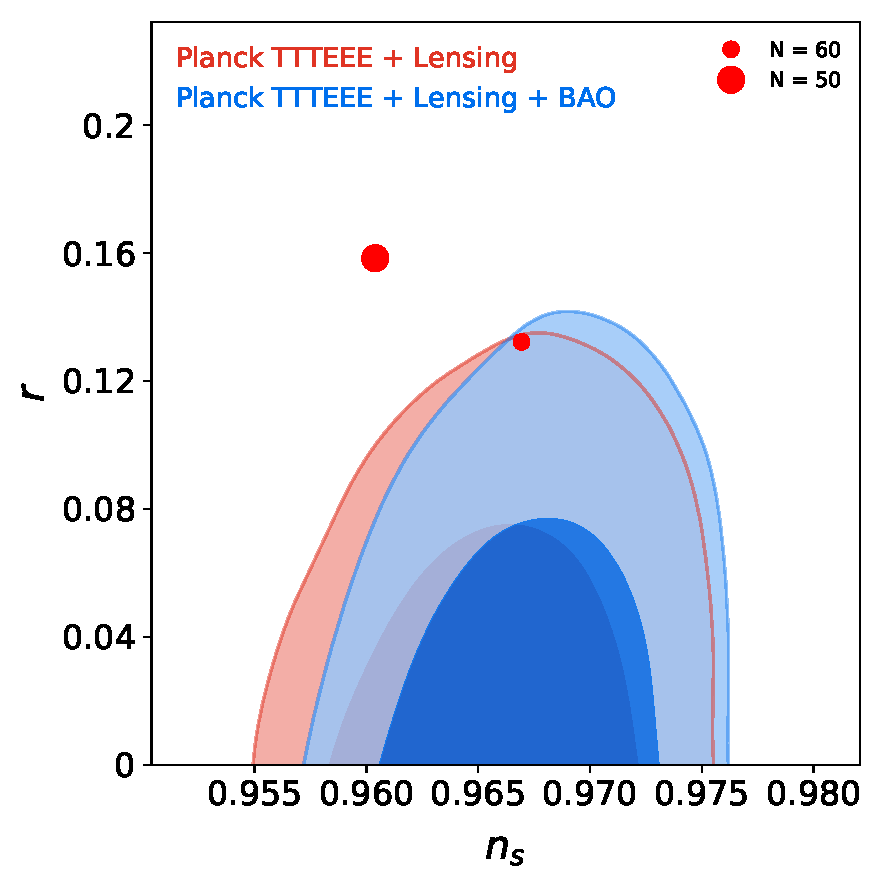
\includegraphics[width=0.6\textwidth]{./figures/fig1.pdf}
\end{subfigure}
\begin{subfigure}[b]{.5\textwidth}
\centering
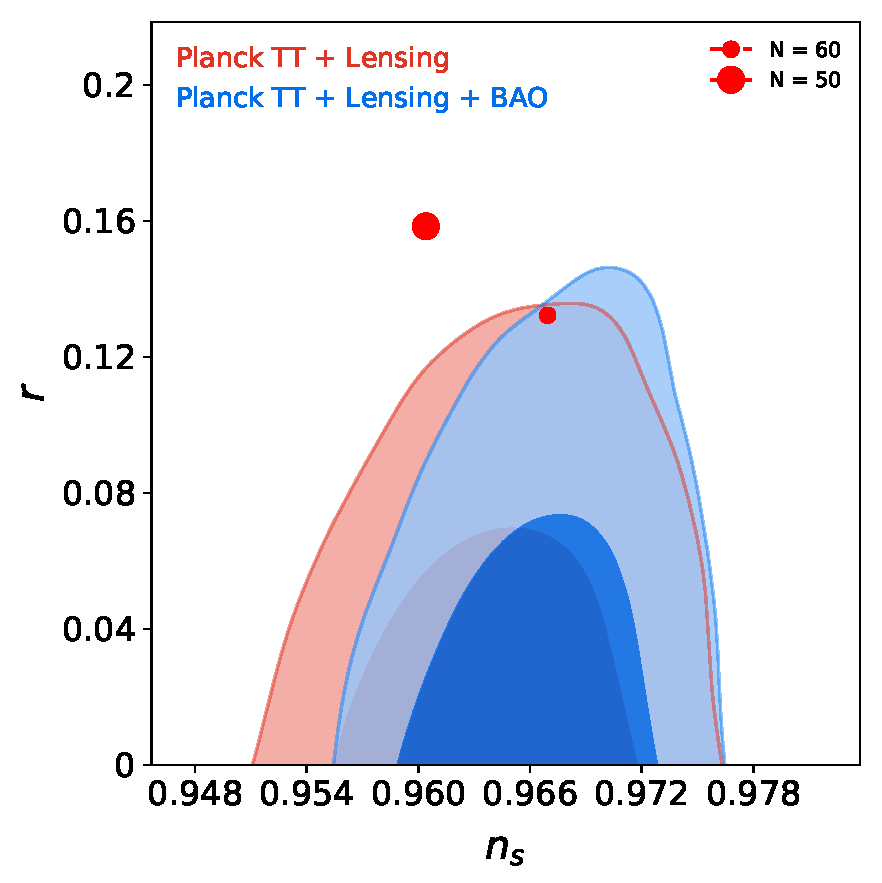
\includegraphics[width=0.6\textwidth]{./figures/fig4.pdf}
\end{subfigure}
\caption{Tensor power spectrum amplitude ($r$)}
\begin{subfigure}[b]{.5\textwidth}
\centering
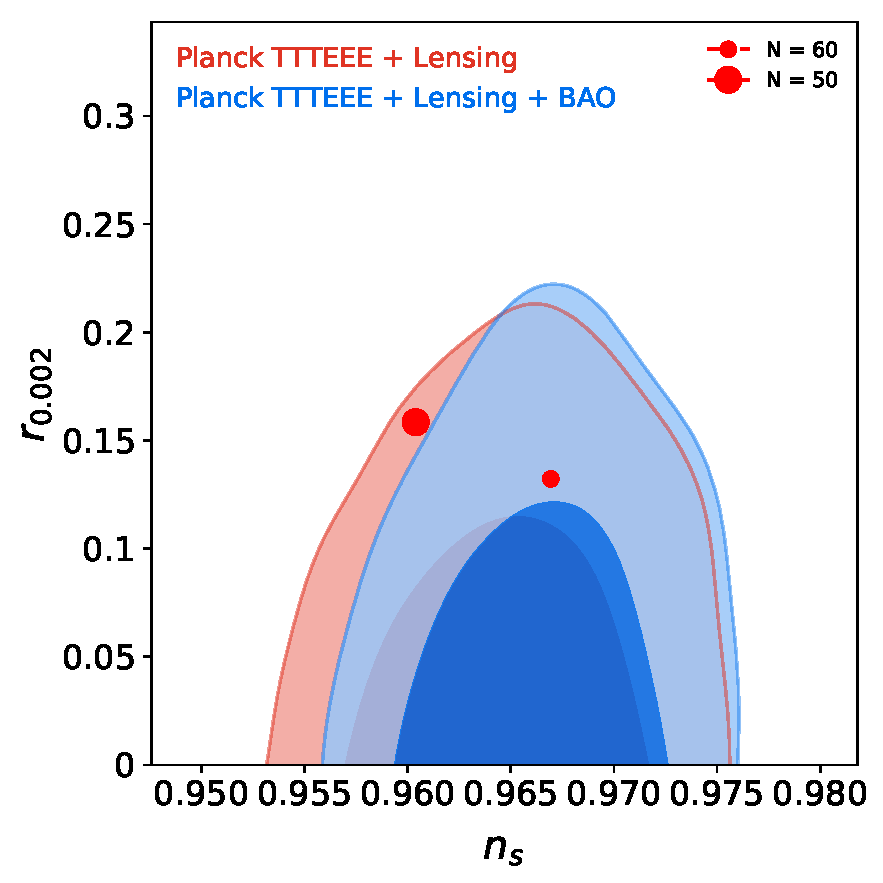
\includegraphics[width=0.6\textwidth]{./figures/fig2.pdf}
\end{subfigure}
\begin{subfigure}[b]{.5\textwidth}
\centering
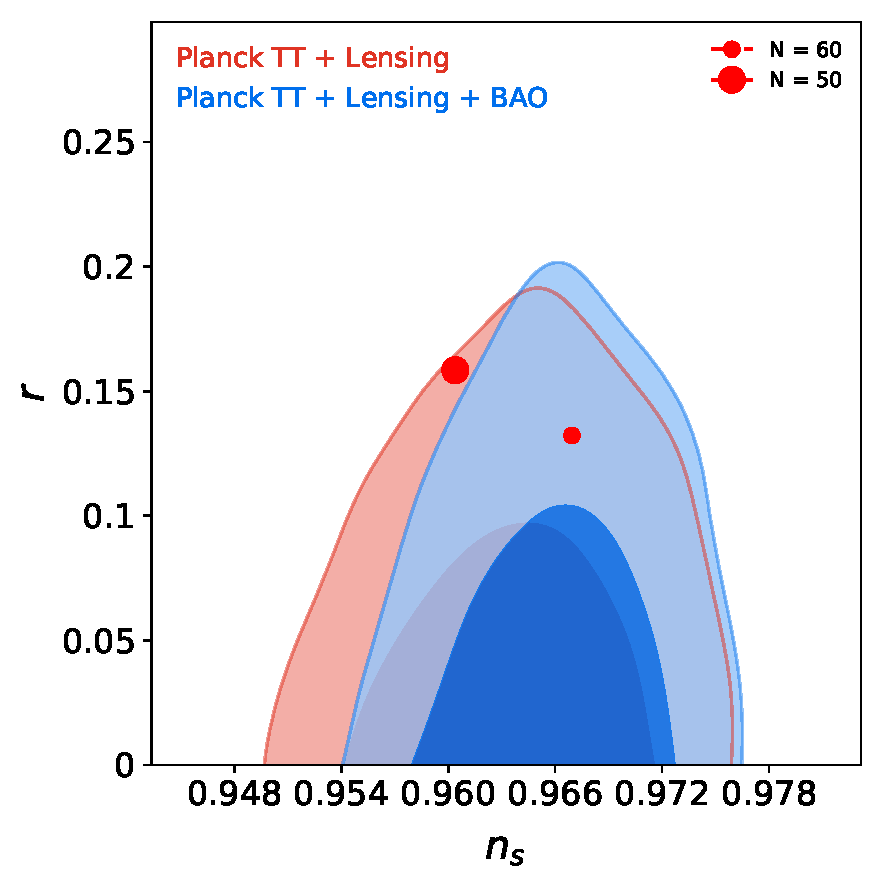
\includegraphics[width=0.6\textwidth]{./figures/fig3.pdf}
\end{subfigure}
\caption{Running of the spectral index + Tensor power spectrum amplitude ($k = 0.05 Mpc^{-1}$)(nrun + r)}
\end{figure}

\section{Conformal transformation}
Conformal transformations allows us to convert non-minimally coupled scalar field in Jordan frame into the minimal coupled scalar field in Einstein frame using the following transformation steps,
\begin{align}
& g_{\mu\nu} \quad \rightarrow\quad \tilde{g}_{\mu\nu} = \Omega^{2}g_{\mu\nu}\\
& \Omega = \sqrt{1 - \kappa \xi \phi^{2}}\\
& d\tilde{\phi} = \frac{\sqrt{1 - \kappa \xi \left(1-6\xi\right)\phi^{2}}}{1 - \kappa \xi \phi^{2}}\\
& \tilde{V}\left[\tilde{\phi}\right] = \frac{V\left[\phi\left(\tilde{\phi}\right)\right]}{\left(1 - \kappa \xi \phi^{2}\right)^{2}}
\end{align}

The action which represents the dynamics of the non-minimally coupled scalar field in Jordan frame is given as,
\begin{align}
S = \int d^{4}x \sqrt{-g}\left[\frac{M_{p}^{2}}{2}R + \frac{\xi}{2}R\phi^{2} - \frac{1}{2}\left(\partial\phi\right)^{2} - U\left(\phi\right)\right]
\end{align}



\section{Non-minimal coupling in Einstein frame}

\end{document}
